\documentclass{minimal}
\usepackage{epsfig,color}
\usepackage{units}
\usepackage[papersize={576.00bp,432.00bp},text={576.00bp,432.00bp}]{geometry}
\begin{document}
\centering
% Title: glps_renderer figure
% Creator: GL2PS 1.3.8, (C) 1999-2012 C. Geuzaine
% For: Octave
% CreationDate: Wed Oct 29 20:18:43 2014
\setlength{\unitlength}{1pt}
\begin{picture}(0,0)
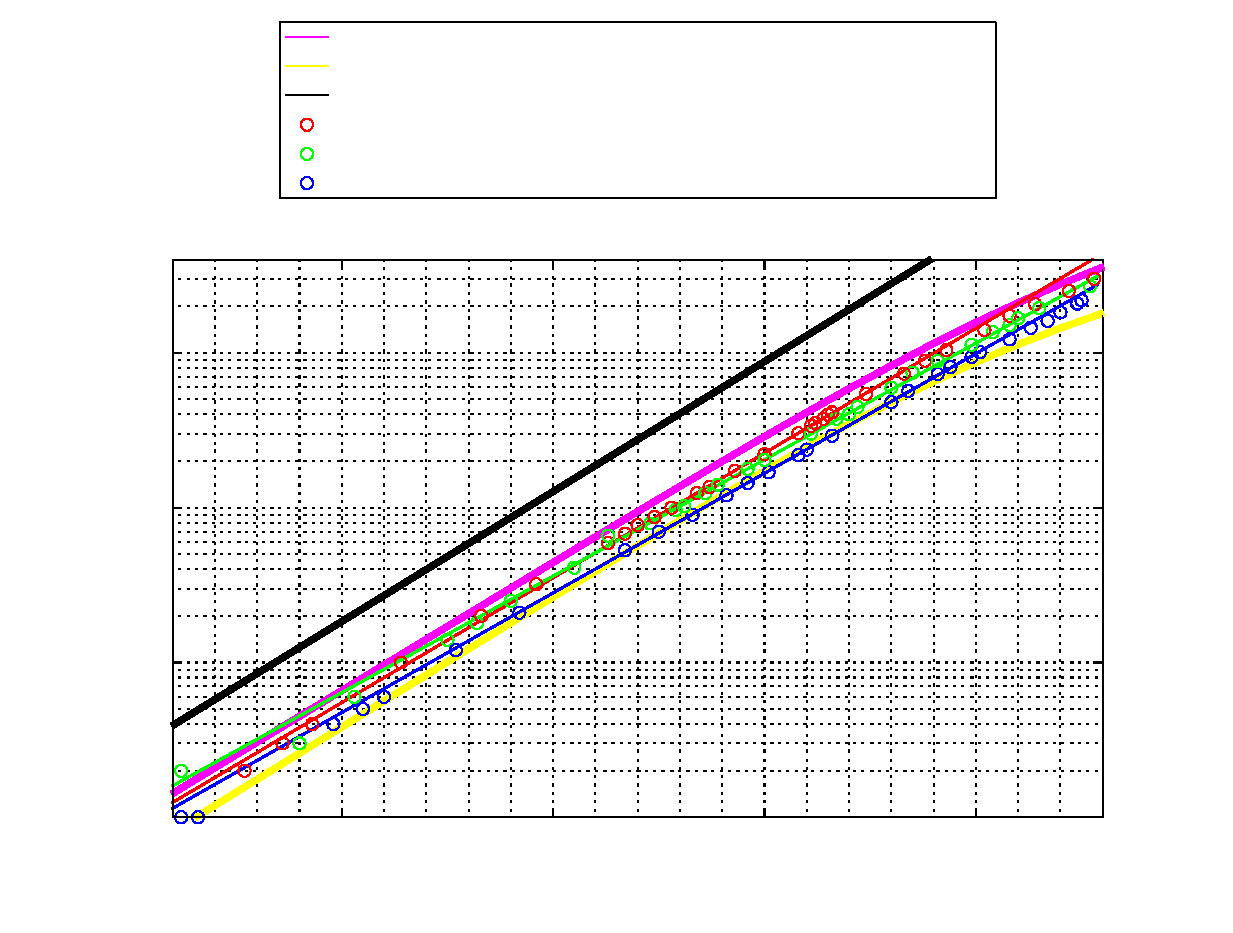
\includegraphics{IdvsVbe_exp-inc}
\end{picture}%
\begin{picture}(576,432)(0,0)
\fontsize{10}{0}
\selectfont\put(156.044,42.5252){\makebox(0,0)[t]{\textcolor[rgb]{0,0,0}{{550}}}}
\fontsize{10}{0}
\selectfont\put(257.498,42.5252){\makebox(0,0)[t]{\textcolor[rgb]{0,0,0}{{600}}}}
\fontsize{10}{0}
\selectfont\put(358.953,42.5252){\makebox(0,0)[t]{\textcolor[rgb]{0,0,0}{{650}}}}
\fontsize{10}{0}
\selectfont\put(460.407,42.5252){\makebox(0,0)[t]{\textcolor[rgb]{0,0,0}{{700}}}}
\fontsize{10}{0}
\selectfont\put(69.8755,47.52){\makebox(0,0)[r]{\textcolor[rgb]{0,0,0}{{1e-2}}}}
\fontsize{10}{0}
\selectfont\put(69.8755,121.844){\makebox(0,0)[r]{\textcolor[rgb]{0,0,0}{{1e-1}}}}
\fontsize{10}{0}
\selectfont\put(69.8755,196.168){\makebox(0,0)[r]{\textcolor[rgb]{0,0,0}{{1e+0}}}}
\fontsize{10}{0}
\selectfont\put(69.8755,270.492){\makebox(0,0)[r]{\textcolor[rgb]{0,0,0}{{1e+1}}}}
\fontsize{10}{0}
\selectfont\put(298.08,31.5252){\makebox(0,0)[t]{\textcolor[rgb]{0,0,0}{{$V_{BE} [\unit{mV}]$}}}}
\fontsize{10}{0}
\selectfont\put(39.8755,181.38){\rotatebox{90}{\makebox(0,0)[b]{\textcolor[rgb]{0,0,0}{{$I_C [\unit{mA}]$}}}}}
\fontsize{10}{0}
\selectfont\put(152.378,422.224){\makebox(0,0)[l]{\textcolor[rgb]{0,0,0}{{\texttt{PHIL\_BJT} $I_S = 57,60122\unit{pA}$  $V_{th}= 26,36066\unit{mV}$}}}}
\fontsize{10}{0}
\selectfont\put(152.378,408.164){\makebox(0,0)[l]{\textcolor[rgb]{0,0,0}{{\texttt{SIEMENS} $I_S = 29,87850\unit{pA}$  $V_{th}= 26,20057\unit{mV}$}}}}
\fontsize{10}{0}
\selectfont\put(152.378,394.104){\makebox(0,0)[l]{\textcolor[rgb]{0,0,0}{{modelo propio $I_S = 107,5609\unit{pA}$ $V_{th} = 25,86963\unit{mV}$}}}}
\fontsize{10}{0}
\selectfont\put(152.378,380.044){\makebox(0,0)[l]{\textcolor[rgb]{0,0,0}{{transistor 1 $I_S = 75,51927\unit{pA}$  $V_{th}= 26,95065\unit{mV}$}}}}
\fontsize{10}{0}
\selectfont\put(152.378,365.984){\makebox(0,0)[l]{\textcolor[rgb]{0,0,0}{{transistor 2 $I_S = 339,5251\unit{pA}$  $V_{th}= 28,86619\unit{mV}$}}}}
\fontsize{10}{0}
\selectfont\put(152.378,351.924){\makebox(0,0)[l]{\textcolor[rgb]{0,0,0}{{transistor 3 $I_S = 150,4921\unit{pA}$  $V_{th}= 28,10407\unit{mV}$}}}}
\end{picture}
\end{document}
